\documentclass[11pt,a4paper]{article}
\usepackage[T1]{fontenc}
\usepackage[utf8]{inputenc}
\usepackage{lmodern}
\usepackage[margin=2.5cm]{geometry}
\usepackage{microtype}
\usepackage{amsmath}
\usepackage{booktabs}
\usepackage{graphicx}
\usepackage{caption}
\usepackage{subcaption}
\usepackage{threeparttable}
\usepackage[authoryear,round]{natbib}
\usepackage{xcolor}
\usepackage[colorlinks=true,linkcolor=blue!50!black,citecolor=blue!50!black,urlcolor=blue!50!black]{hyperref}
\usepackage{setspace}
\usepackage[section]{placeins}
\setstretch{1.08}
\captionsetup{font=small,labelfont=bf,margin=0.5cm}
\graphicspath{{../empirics/results/figures/}}
\newcommand{\figwidth}{0.92\textwidth}

\title{\textbf{Sanctions and Russian Invention}\\[0.3em]
\large EU export bans, import substitution and domestic patents by technology field}
\author{Fyodor Shafranov\thanks{LMU Munich. Work in progress; not for citation. All numbers are from the
replication package in this repository (\texttt{run\_all.sh}); data decisions are logged in
\texttt{notes/data\_decisions.md}.}}
\date{12 November 2026 --- draft report}

\begin{document}
\maketitle

\begin{abstract}
\noindent
After February 2022 the European Union banned the export to Russia of goods that accounted for half of Russia's
pre-war Western imports of manufactured goods. Did Russian inventors respond by substituting for the lost
technologies, or did domestic invention fall where imported inputs were cut? I combine the Rospatent register of
granted inventions, a title-based classifier that assigns technology fields to patents after 2018, Russia's
product-level imports from CEPII BACI, and every consolidated version of the EU sanctions regulation since 2014.
The share of a field's pre-war Western imports covered by EU bans strongly predicts the collapse of those imports
(correlation $-0.9$ across 35 fields), and China did not replace more in banned fields. In a pre-registered test,
one standard deviation more ban coverage is associated with 9\% fewer domestic patents in the field after 2022
(95\% CI $[-11.4, -6.9]$\%, randomization $p=0.007$). The pre-period is not flat: banned fields were already
drifting down relative to others. Trend-adjusted and staggered estimates range from $-2$\% to $-15$\%. Across all
specifications, substitution into banned technologies larger than about $+3$\% per standard deviation is ruled
out. Together with a 50--60\% fall in foreign patent filings in Russia, the evidence points to complementarity
between imported inputs and domestic invention, not import substitution.
\end{abstract}

\section{Question}

Sanctions are meant to cut a target economy off from technology. Whether they reduce its capacity to innovate
is less obvious. Two forces work in opposite directions.
\begin{itemize}\setlength\itemsep{0.1em}
  \item \textbf{Substitution.} A ban raises the domestic return to inventing what can no longer be imported.
  Russia's state ``import substitution'' and ``technological sovereignty'' programmes are built on this idea, and
  \citet{LiuLiuMakarinWen2025} find that the 2007 US export controls on China \emph{raised} Chinese patenting in
  the controlled technologies.
  \item \textbf{Complementarity.} Domestic research uses imported equipment, components, materials and software.
  Cutting these off makes invention in the affected technologies harder, as losing access to frontier
  knowledge lowered scientific output after the First World War \citep{IariaSchwarzWaldinger2018}.
\end{itemize}
The 2022 sanctions on Russia are an unusually large and well documented test. The bans were broad, written by
the sanctioning side, dated in law, and varied sharply across technologies: telecom equipment and semiconductors
were mostly banned, medicines and medical devices mostly exempt. This report uses that variation to ask whether
domestic invention moved \emph{toward} or \emph{away from} the technologies that were cut off.

\section{Data}

\paragraph{Patents.} The Rospatent open register of granted inventions (version of 2 November 2026; 867,684
patents) gives application dates, holders, authors, correspondence addresses and titles, but no technology
classes. Domestic patents are those whose holders are all Russian and that claim no foreign priority (65\% of
grants filed since 2000). Four individual mass filers are dropped; one of them alone held about 14\% of
Russian invention grants in 2005--2015 (canning recipes). Patents are dated by filing year. Grant lags are now
short: domestic grants by filing year are about 15,000--16,800 for 2019--2024, so 2022--2024 filings are close
to complete; 2025 is incomplete.

\paragraph{Technology fields.} The 35 fields of the WIPO technology concordance \citep{Schmoch2008}. For patents
filed up to 2017, IPC codes come from Google Patents (BigQuery), matched on registration number (96--99\%
coverage). After 2018 the match rate collapses (71\% for 2020, 39\% for 2021, about 0 from 2022), so fields are
imputed from titles (Section~\ref{sec:classifier}).

\paragraph{Trade.} CEPII BACI \citep{GaulierZignago2010}, HS 2007, release January 2026 (2007--2024). BACI
reconciles importer and exporter reports, so Russia's imports after 2021 are measured from partners' exports. The
West is the 2022 sanctions coalition (EU27, US, UK, Canada, Japan, Korea, Taiwan, Singapore, Australia, New
Zealand, Switzerland, Norway, Iceland, Liechtenstein). The West's share of Russia's imports fell from 60\%
(2011--13) to 49\% (2021) and 22\% (2024); imports from China rose from \$73bn (2021) to \$115bn (2024).

\paragraph{Products to fields.} Two independent maps from HS 6-digit products to the 35 fields, used to check
each other:
(i) the title classifier applied to the Russian product names of the EAEU customs tariff (TN VED); and
(ii) HS $\to$ ISIC Rev.4 \citep[R package \texttt{concordance}]{concordance} $\to$ NACE Rev.2 $\to$ fields, using the
industry--technology table of \citet{DornerHarhoff2018}, estimated from German inventors linked to their
employers. Both maps cover 99\% of import value.

\paragraph{Sanctions.} All 35 consolidated versions of Council Regulation (EU) No 833/2014 (September 2014 to
July 2026), from the EU Publications Office's CELLAR API. I parse every export-ban annex that lists customs codes:
industrial goods (Annex XXIII and its parts, the bulk), oil refining (X), aviation and space (XI), jet fuel (XX),
luxury goods (XVIII), firearms (XXXV) and, from December 2023, the G7 Common High Priority List (XL). For 2014,
Annex II (oil-industry equipment) is used. Codes are converted to HS 2007 using the HS vintage in force at each
version date. Annex VII (advanced technology) defines items by technical description, without customs codes; its
electronics enter only through Annex XL and are therefore dated too late (December 2023).

\section{Measuring technology fields after 2018}\label{sec:classifier}

Fields for post-2018 patents are imputed from the Russian title with a TF-IDF representation (word 1--2-grams
and character 3--5-grams, which handle Russian inflection) and a multinomial logistic regression, trained on
581,000 patents with both a title and IPC codes. Labelled patents get out-of-fold predictions (five-fold
cross-fitting); each patent is counted once in its most likely field. Table~\ref{tab:classifier} summarises the
validation.

\begin{table}[ht]
\centering
\begin{threeparttable}
\caption{Validation of the title classifier}\label{tab:classifier}
\small
\begin{tabular}{lc}
\toprule
Test & Result \\
\midrule
Random 10\% of 2005--17 held out: top-1 / top-3 field correct & 84\% / 96\% \\
Out of time (trained $\le 2017$, tested 2018--21): top-1 / top-3 & 81\% / 95\% \\
Field shares by year, predicted vs IPC (2018--21): correlation & 0.994--0.998 \\
Within-field changes, field and year FE, 2010--20: correlation / slope & 0.91 / 0.93 \\
Same with summed probabilities instead of top field: slope & 0.55 \\
\bottomrule
\end{tabular}
\begin{tablenotes}\footnotesize
\item Notes: ``Correct'' = the predicted field is among the patent's IPC-based fields. The last two rows compare
domestic patent counts by field and year built from predicted and from true fields, after removing field and year
fixed effects; a slope near 1 means the imputation does not attenuate event-study coefficients.
\end{tablenotes}
\end{threeparttable}
\end{table}

The test that matters for this design is the fourth row: year-to-year changes within a field are reproduced with
a slope of 0.93. Counting each patent in its top field matters; summing probabilities shrinks changes toward the
average field and would bias effects toward zero. Eight fields have out-of-time recall below 0.5 (IT methods for
management, micro- and nano-technology, control, surface technology, textile and paper machines, semiconductors,
environmental technology, analysis of biological materials). Figure~\ref{fig:classifier} shows that most of these
differ from the IPC series in level, which field fixed effects absorb; dropping them does not change the results.

\begin{figure}[p]
\centering
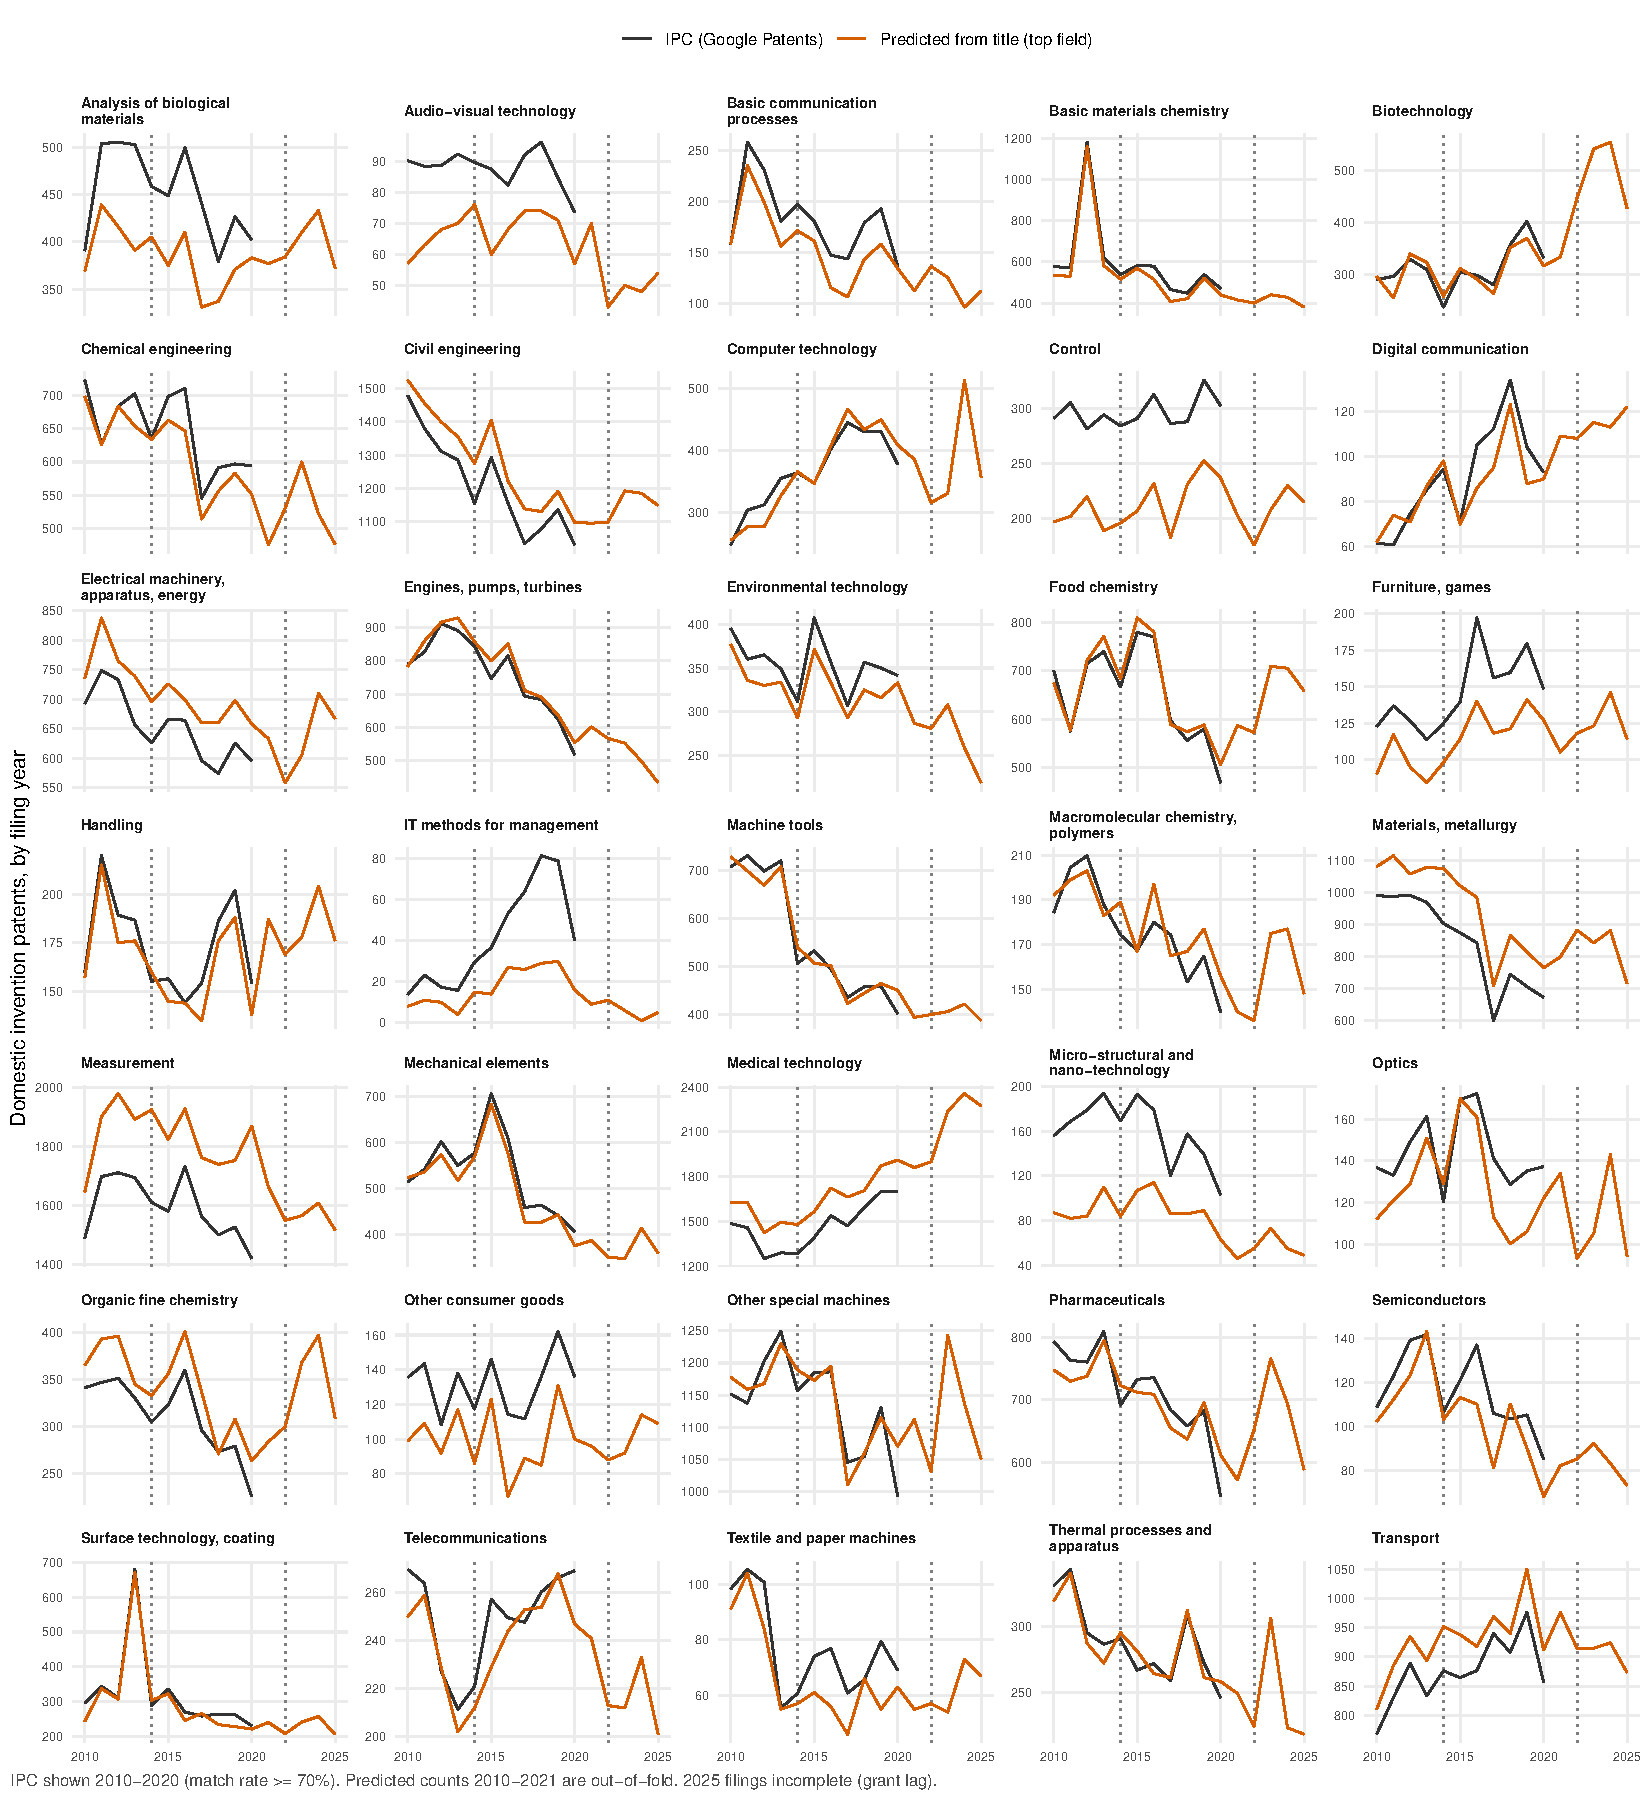
\includegraphics[width=\textwidth]{fig25_title_classifier_fields.pdf}
\caption{Domestic invention patents by WIPO field: IPC-based counts (2010--2020) and counts predicted from titles
(2010--2025). Predicted counts for 2010--2021 are out-of-fold. Dotted lines: 2014 and 2022.}
\label{fig:classifier}
\end{figure}

\section{Treatment: EU ban coverage by technology field}

\subsection{Why the pre-war import share does not work}

The natural exposure measure, the West's share of a field's imports before 2022, fails. It is highest in
pharmaceuticals, medical technology and biotechnology, which were largely exempt from the bans as humanitarian
goods. A higher pre-war Western share therefore predicts a \emph{smaller} loss of Western imports after 2022
(+0.34 log points per SD by 2024, industry map). Exposure has to measure what was actually cut off.

\subsection{Ban coverage}

Following the logic of \citet{KantorWhalley2025}, who define exposure from the rival's demands rather than the
funder's choices, treatment is defined by the sanctioning side. For field $f$ and year $y$,
\begin{equation}
\text{Ban}_{fy} \;=\; \frac{\sum_{h} w_{hf}\, W_h\, b_{hy}}{\sum_{h} w_{hf}\, W_h},
\end{equation}
where $h$ indexes HS 2007 products, $w_{hf}$ is the product-to-field weight, $W_h$ is Russia's average annual
import of $h$ from the West in 2019--21, and $b_{hy}$ is the share of $h$ banned in the last consolidated version
dated by 31 December of year $y$. The main measure is coverage at the end of 2023, z-scored across fields.

Coverage of Western manufactured imports rose from 25\% (end-2022) to 49\% (2023), 57\% (2024) and 65\% (2026).
It is highest in telecommunications, digital communication, semiconductors, computer technology, transport and
engines (58--83\% depending on the map) and lowest in medical technology, pharmaceuticals, analysis of biological
materials and biotechnology (10--35\%). The 2014 oil-equipment list covered only 1.4\% of Western imports and at
most 4\% of any field.

\subsection{First stage}

Figure~\ref{fig:fs} shows the cross-section of fields: ban coverage explains almost all of the variation in the
realised fall of Western imports between 2019--21 and 2023--24 (correlation $-0.94$ with the industry map,
$-0.90$ with the product-name map). In an event study (PPML, field and year fixed effects, base 2021), one SD
more coverage lowers Western imports by $0.31$--$0.48$ log points in 2023 and $0.38$--$0.61$ in 2024, with tight
intervals. Imports from China did not rise disproportionately in banned fields, and total imports fell more
there ($-0.08$ per SD with the product-name map). Banned fields therefore lost supply in net terms, which is the
condition under which import substitution should appear. Two caveats: Western imports into later-banned fields
were somewhat higher in 2015--17 relative to 2021, and BACI probably undercounts re-exports through Central Asia
and the Caucasus.

\begin{figure}[ht]
\centering
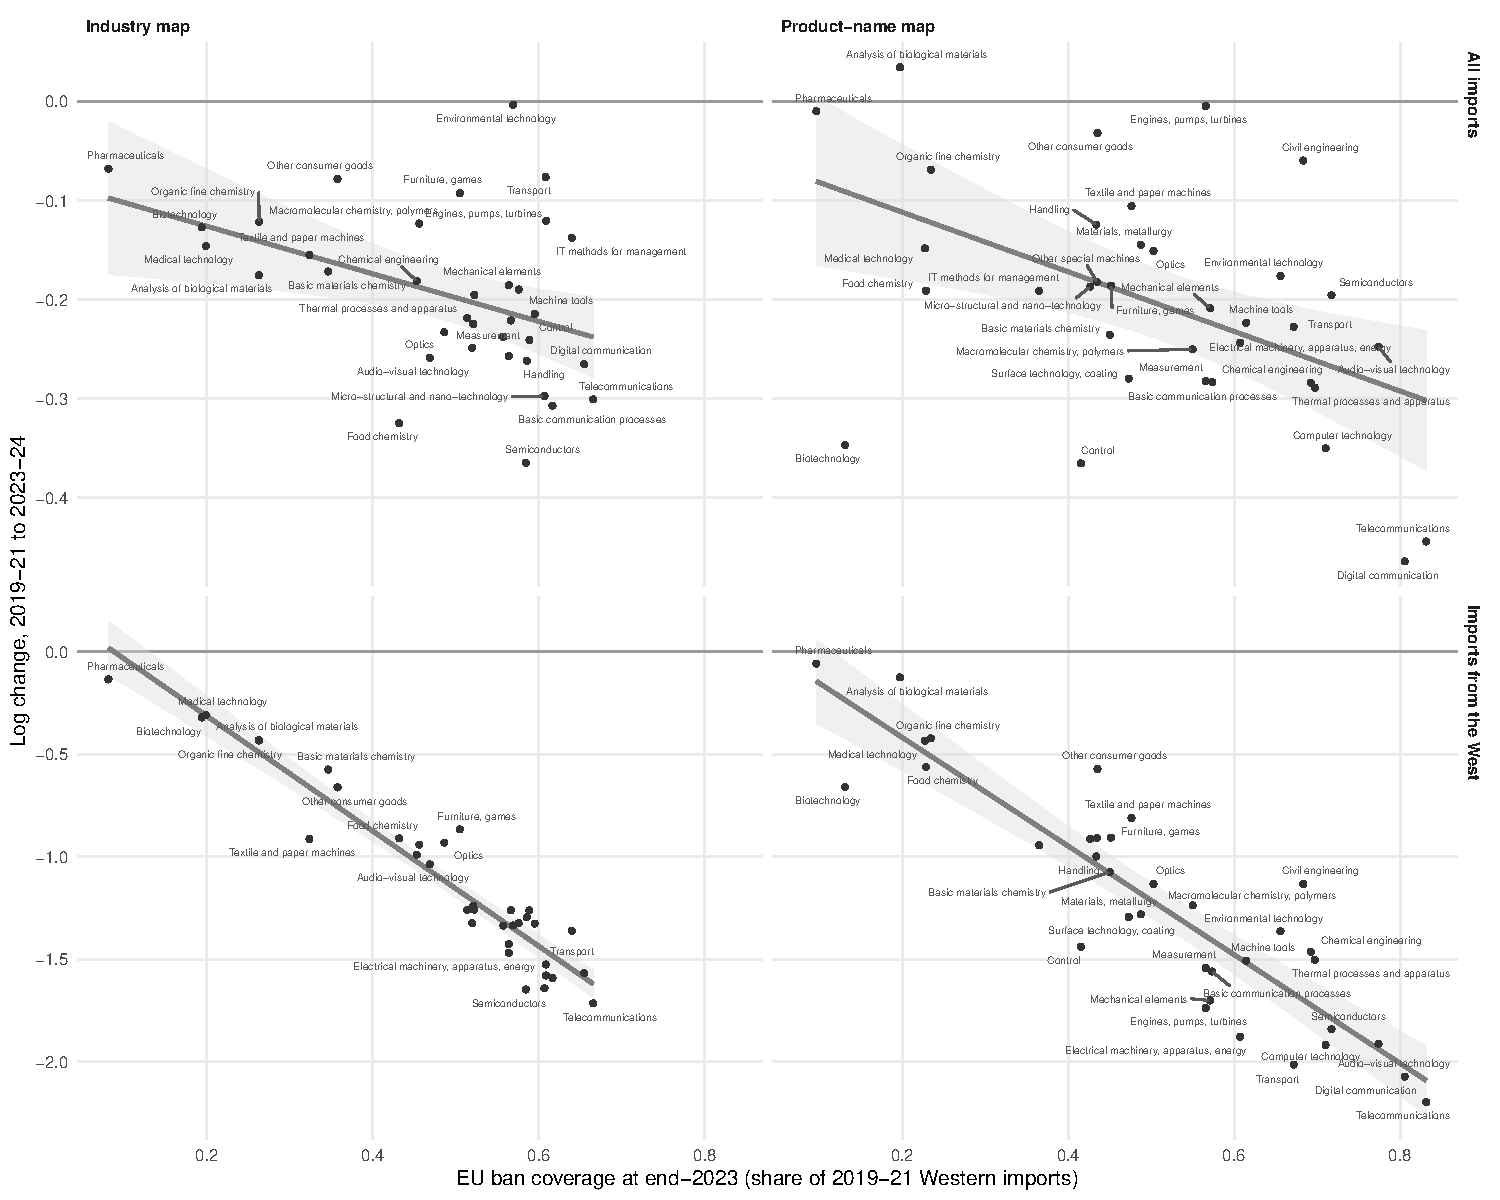
\includegraphics[width=\figwidth]{fig29_ban_coverage_vs_drop.pdf}
\caption{EU ban coverage at end-2023 and the log change in Russia's imports between 2019--21 and 2023--24, by
technology field. Top: all imports. Bottom: imports from the West. Left: industry map; right: product-name map.}
\label{fig:fs}
\end{figure}

\section{Main result}

\subsection{Pre-registered specification}

Before any estimate was computed, the following test and decision rule were written down and committed
(\texttt{notes/11\_patents\_ban\_test.md}):
\begin{equation}
P_{ft} \;=\; \exp\!\big(\beta \cdot \text{Ban}_f \cdot \text{Post}_t \;+\; \alpha_f \;+\; \gamma_t\big)\,\varepsilon_{ft},
\end{equation}
estimated by Poisson pseudo-maximum likelihood on 35 fields $\times$ 2015--2025, where $P_{ft}$ is domestic
invention patents, $\text{Ban}_f$ is end-2023 coverage (industry map, z-scored), and $\text{Post}_t=1$ from 2022.
Standard errors are clustered by field; the main $p$-value comes from randomization inference, permuting
$\text{Ban}_f$ across fields 2,000 times. The industry map is the main version because the product-name map uses
the same classifier as the outcome. Import substitution predicts $\beta>0$.

\subsection{Result}

The estimate is $\hat\beta = -0.092$ (95\% CI $[-0.114, -0.069]$; randomization $p=0.0065$, Figure~\ref{fig:ri}).
One SD of coverage is about 13 percentage points of a field's Western imports. Comparing telecommunications
(coverage 0.65) with pharmaceuticals (0.25), about three SD apart, implies roughly 25\% fewer domestic patents in
telecommunications after 2022, relative to pharmaceuticals. All six pre-specified robustness checks have the same
sign (Table~\ref{tab:main}). The decline is clearest for research institutes and universities; for firms it is
smaller and the interval just includes zero.

\begin{table}[ht]
\centering
\begin{threeparttable}
\caption{Domestic patents and EU ban coverage: pre-registered test and robustness}\label{tab:main}
\small
\begin{tabular}{lccc}
\toprule
Specification & $\hat\beta$ & 95\% CI & Fields \\
\midrule
\textbf{Main} (industry map, 2015--2025) & $\mathbf{-0.092}$ & $[-0.114, -0.069]$ & 35 \\
\quad Randomization inference ($p$) & \multicolumn{3}{l}{0.0065 (2,000 permutations)} \\
\addlinespace
1. Product-name map & $-0.099$ & $[-0.154, -0.045]$ & 35 \\
2. Drop weak classifier fields & $-0.090$ & $[-0.114, -0.066]$ & 27 \\
3a. Firms only & $-0.047$ & $[-0.101, +0.007]$ & 35 \\
3b. Universities only & $-0.091$ & $[-0.122, -0.061]$ & 35 \\
3c. Research institutes only & $-0.118$ & $[-0.149, -0.087]$ & 35 \\
4. IPC where available, predicted otherwise & $-0.090$ & $[-0.111, -0.069]$ & 35 \\
5. Years 2015--2024 & $-0.087$ & $[-0.108, -0.065]$ & 35 \\
6. Coverage without partial (``ex'') bans & $-0.090$ & $[-0.114, -0.065]$ & 35 \\
\bottomrule
\end{tabular}
\begin{tablenotes}\footnotesize
\item Notes: PPML of domestic invention patents by field and filing year on $\text{Ban}_f \times \text{Post}_t$
with field and year fixed effects. $\text{Ban}_f$ is z-scored; coefficients are log points per SD. Standard
errors clustered by field.
\end{tablenotes}
\end{threeparttable}
\end{table}

\begin{figure}[ht]
\centering
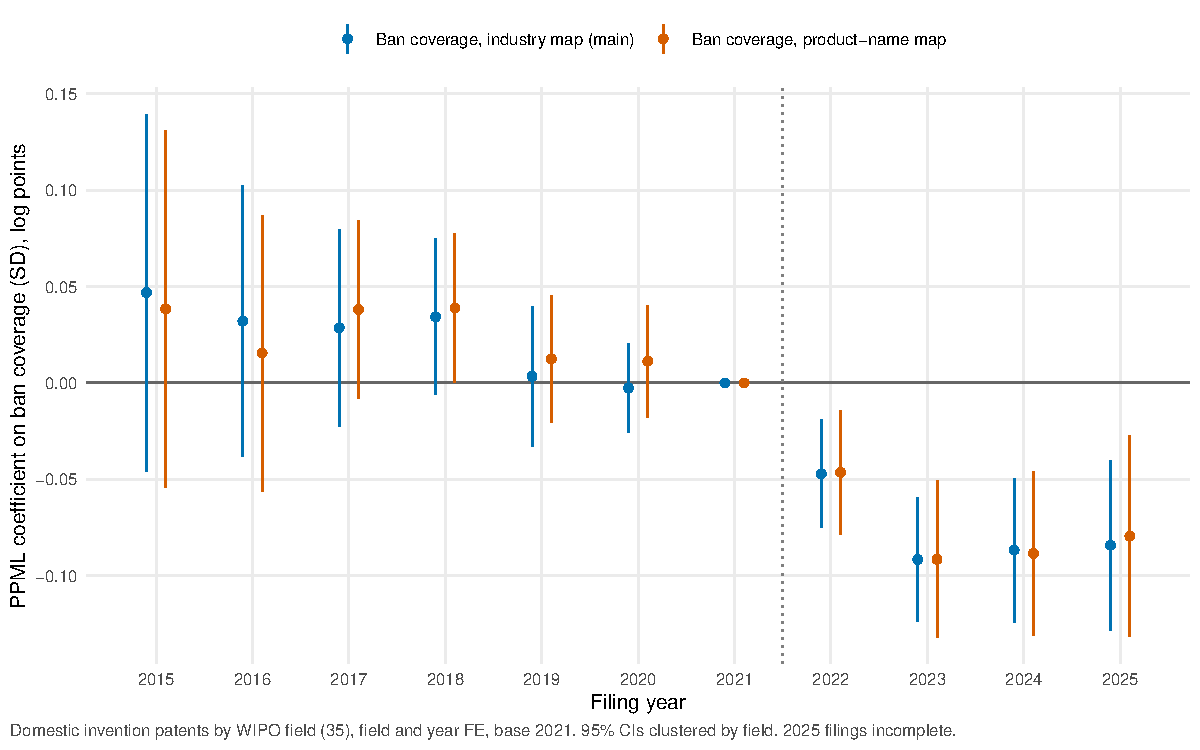
\includegraphics[width=\figwidth]{fig30_patents_ban_eventstudy.pdf}
\caption{Event study: domestic invention patents on EU ban coverage (SD) $\times$ year, PPML with field and year
fixed effects, base 2021. 95\% confidence intervals clustered by field. 2025 filings are incomplete.}
\label{fig:es}
\end{figure}

\section{Pre-trends}

The event study (Figure~\ref{fig:es}) does not have a flat pre-period. Relative to 2021, high-coverage fields
had more patents in 2015--2018 (+0.04 to +0.06 per SD), with 2017 and 2018 excluding zero, and 2019--2021 is
flat. Banned fields were therefore drifting down relative to other fields by about 1\% per SD per year before the
sanctions, broadly a shift of Russian invention from machinery and electronics toward life sciences. By the
decision rule written in advance, the sign can be read but the size cannot be taken from the main estimate.

The drift runs in the same direction as the effect, so a continuing trend could explain part of the post-2022
decline. Table~\ref{tab:trends} reports exploratory checks that were not pre-registered.

\begin{table}[ht]
\centering
\begin{threeparttable}
\caption{Exploratory trend checks (not pre-registered)}\label{tab:trends}
\small
\begin{tabular}{lcc}
\toprule
Specification & Industry map (main) & Product-name map \\
\midrule
Unadjusted (main test) & $-0.092$ $[-0.114, -0.069]$ & $-0.099$ $[-0.154, -0.045]$ \\
Window 2019--2025 (flat pre-period) & $-0.066$ $[-0.085, -0.047]$ & $-0.084$ $[-0.120, -0.049]$ \\
Field-specific linear trends & $-0.027$ $[-0.080, +0.027]$ & $-0.064$ $[-0.121, -0.007]$ \\
Extrapolated linear pre-trend in the ban gradient & $-0.021$ $[-0.074, +0.032]$ & $-0.060$ $[-0.117, -0.003]$ \\
\bottomrule
\end{tabular}
\begin{tablenotes}\footnotesize
\item Notes: PPML, field and year fixed effects, standard errors clustered by field; log points per SD of ban
coverage.
\end{tablenotes}
\end{threeparttable}
\end{table}

Two conclusions follow. First, no specification produces a positive estimate; the highest upper bound is about
$+0.03$ per SD, so substitution into banned technologies of more than about 3\% per SD is ruled out. Second, the
size of the decline is uncertain: from $-2$\% to $-9$\% per SD depending on how the pre-period drift is treated,
with the trend-adjusted interval including zero for the main map. Insignificant pre-period coefficients are only
a proxy for parallel trends \citep{Roth2022}; the next step is to obtain a flat pre-period by design, comparing
fields within broad sectors, and to report bounds in the spirit of \citet{RambachanRoth2023}.

\begin{figure}[ht]
\centering
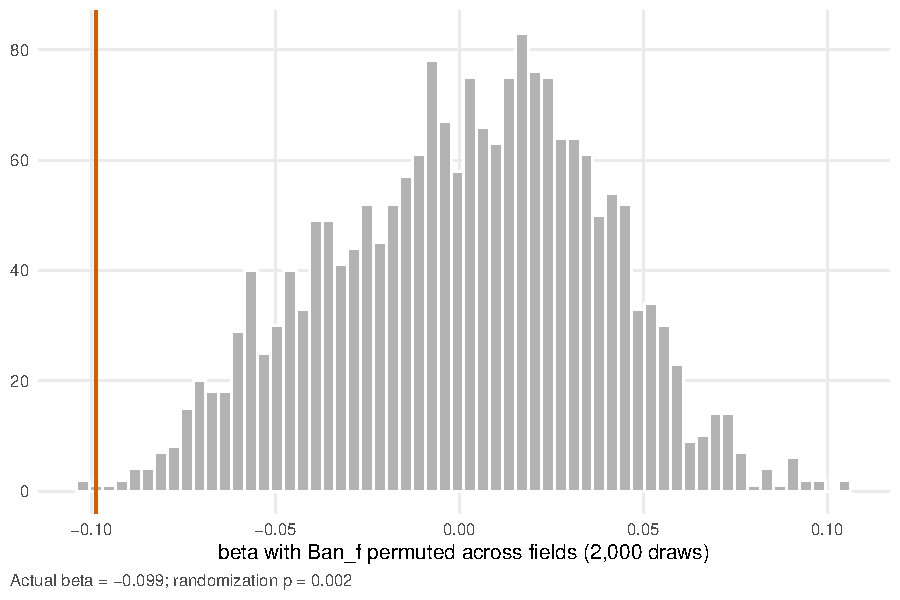
\includegraphics[width=0.62\textwidth]{fig31_patents_ban_ri.pdf}
\caption{Randomization inference: distribution of $\hat\beta$ when ban coverage is permuted across the 35 fields
(2,000 draws), and the actual estimate.}
\label{fig:ri}
\end{figure}

\section{2014 and staggered timing}

\paragraph{2014.} The 2014 export controls were narrow (oil-industry equipment) and coincided with the collapse
of the oil price and the rouble. With the 2014 list as exposure, patents in affected fields show a flat
pre-period and a mild relative decline from 2016 ($-0.05$ in 2016 and $-0.07$ in 2017 per SD, both excluding
zero), which cannot be separated from the oil-price shock. Fields that were later banned in 2022 show no reaction
around 2014 at all (Figure~\ref{fig:2014}, lower panel): neither the devaluation nor the import-substitution
programmes from 2015 pulled invention into import-dependent fields. Their slow relative decline starts around
2016 and steepens in 2022.

\paragraph{Continuous dose.} Letting coverage vary by field and year over 2008--2025 (the oil list from 2014,
the EU lists from 2022), banning another 10 percentage points of a field's Western imports is associated with
7.6\% fewer domestic patents ($[-10.0, -5.3]$\%). The 2014 list adds no information because its coverage never
exceeds 4 percentage points.

\paragraph{Staggered adoption.} The EU added products package by package, so fields reached high coverage in
different years. Defining a field as treated from the first year its coverage reaches 50\% gives cohorts of 21
(2023), 5 (2024) and 4 (2025) fields, with 5 never treated by 2025. Heterogeneity-robust estimators give
$-0.105$ $[-0.19, -0.02]$ \citep[PPML]{SunAbraham2021} and $-0.125$ to $-0.147$
\citep[log outcome, never- and not-yet-treated controls]{CallawaySantAnna2021}; plain TWFE gives about twice
that ($-0.22$). With a 60\% threshold the robust estimates are smaller and their intervals include zero. The
relative-time event study (Figure~\ref{fig:stag}) shows the same pre-period drift as the main test.

\begin{figure}[ht]
\centering
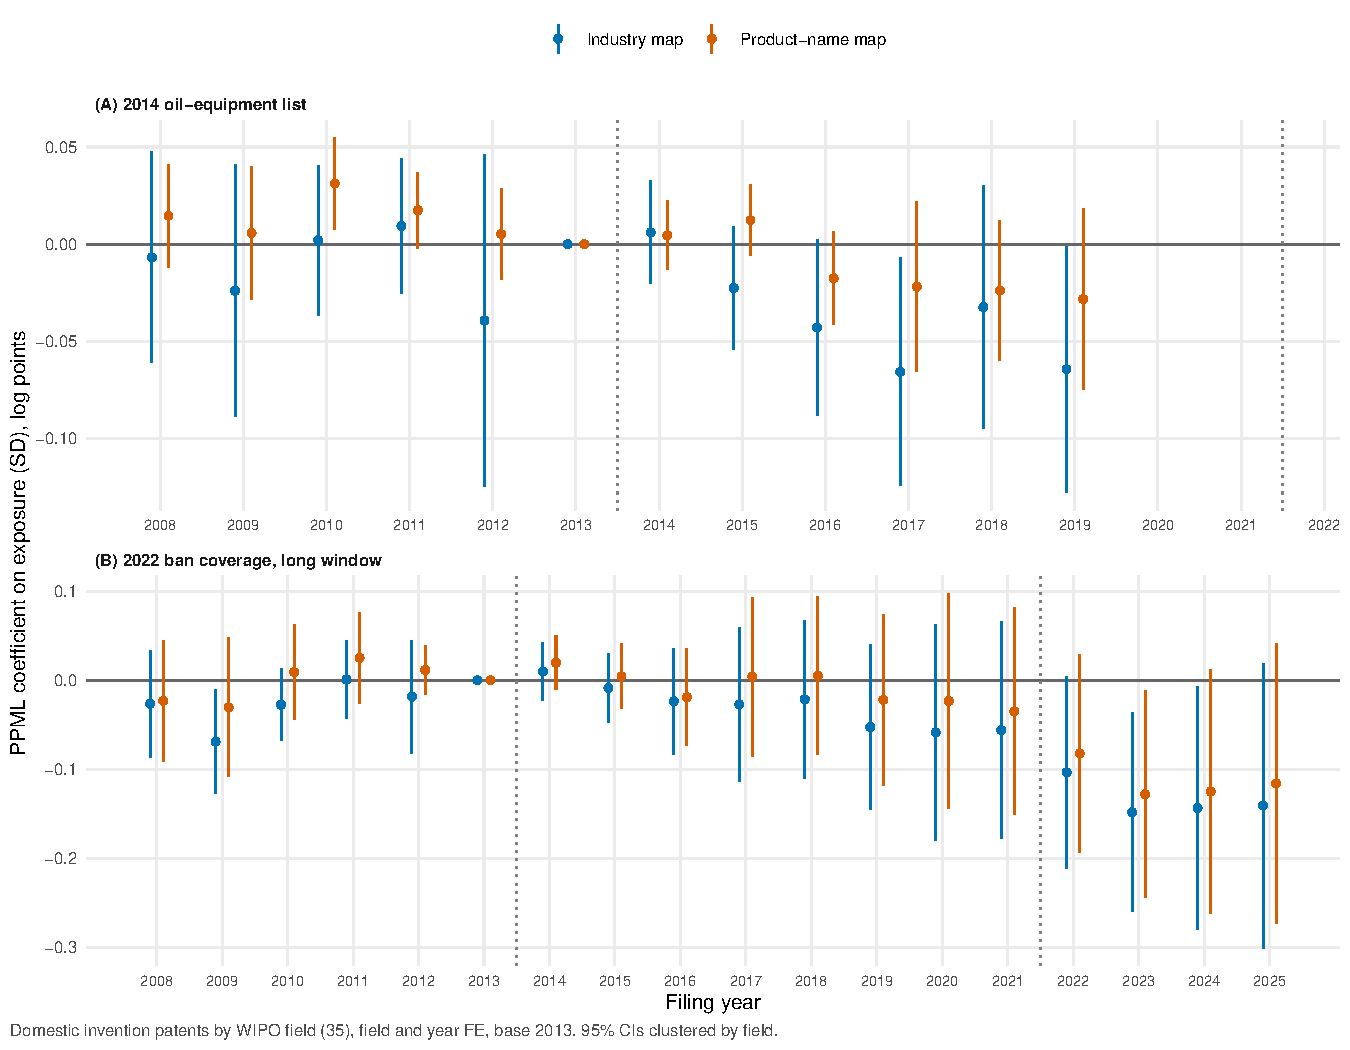
\includegraphics[width=\figwidth]{fig32_patents_2014_eventstudy.pdf}
\caption{Event studies around 2014, base 2013. Top: coverage by the 2014 oil-equipment list (Annex II). Bottom:
EU ban coverage of 2022 over the long window 2008--2025. PPML, field and year fixed effects, 95\% CIs clustered by
field.}
\label{fig:2014}
\end{figure}

\begin{figure}[ht]
\centering
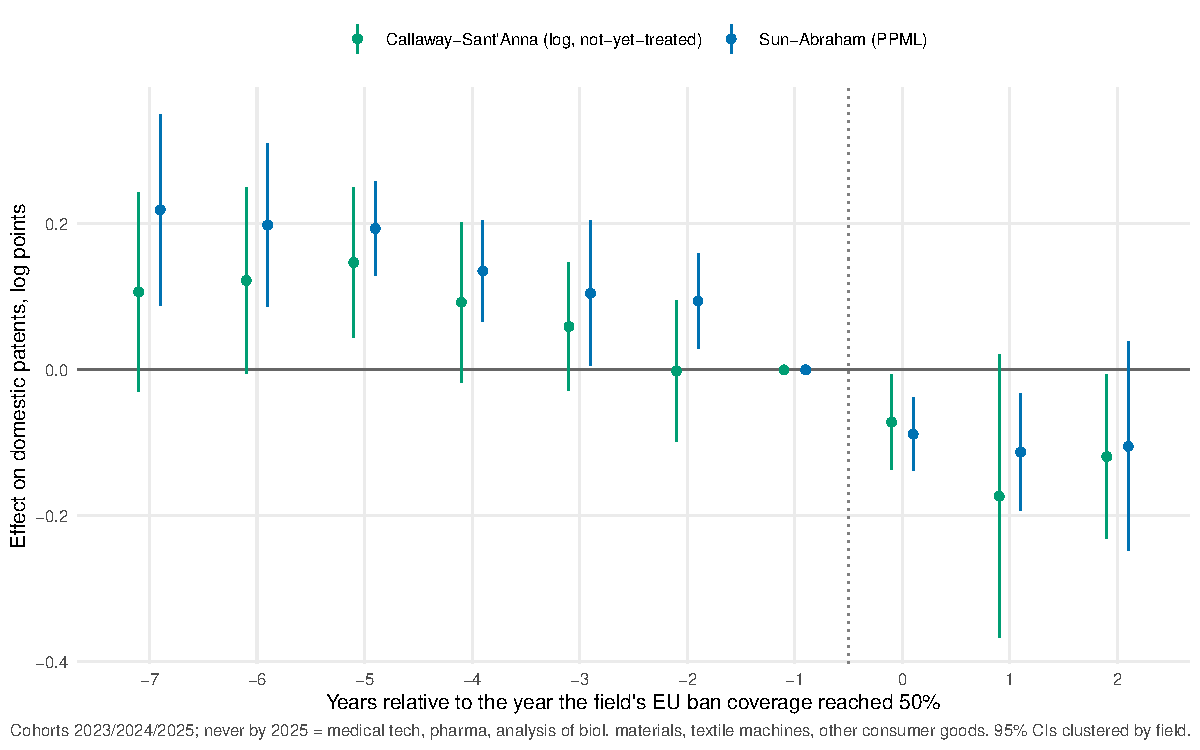
\includegraphics[width=0.85\textwidth]{fig33_patents_staggered.pdf}
\caption{Staggered event study by years relative to the year a field's EU ban coverage reached 50\%:
Sun--Abraham (PPML) and Callaway--Sant'Anna (log outcome, not-yet-treated controls). 95\% CIs clustered by
field.}
\label{fig:stag}
\end{figure}

\section{Context: what else the project found}

The field design is the last of several. Their results are consistent with it.
\begin{itemize}\setlength\itemsep{0.1em}
  \item \textbf{Cross-country.} Staggered DiD over sanctions episodes since 1995 and synthetic DiD for Russia 2014,
  Russia 2022 and Iran 2012 show no robust effect on resident patents, publications or TFP.
  \item \textbf{Foreign filers left.} Non-resident patent filings in Russia fell by $-0.59$ log points after 2022
  against a synthetic control (placebo $p=0.05$), and similarly in Iran after 2012 ($-0.68$). In the raw data,
  foreign filings in Russia fell 54\% between 2021 and 2024.
  \item \textbf{Totals.} Domestic patents in Russia were flat after 2022 (+2\% in 2022--24 vs 2019--21);
  university patents rose 19\%, in line with ministry targets.
  \item \textbf{Regions.} Regions with more Western co-invention or co-authorship did not lose patents or papers
  after 2022, although those links fell by a third or more. After 2014, firm patents rose by 5--10\% per SD in
  regions with Western co-inventors, a suggestive pattern with some pre-trend.
\end{itemize}

\paragraph{Related work.} \citet{EgorovEtAl2026} use hand-collected product-level sanctions on Russia and
customs data and find that sanctioned imports fell sharply, rerouting offset about two-thirds, and firms that
relied on soon-to-be-sanctioned imports lost about 12\% of output; they do not study invention.
\citet{LiuLiuMakarinWen2025} find that narrow US export controls on China in 2007 raised patenting in controlled
technologies by about 65\%. \citet{HovhannisyanMiromanova2025} relate sanctions episodes to Russian patent counts
at the national level. This report combines product-level, sender-defined treatment with invention by
technology field, and finds the opposite of the China result for broad coalition bans.

\section{Limitations and next steps}

\begin{enumerate}\setlength\itemsep{0.1em}
  \item \textbf{Pre-trend.} Obtain a flat pre-period by design: sector $\times$ year fixed effects (WIPO's five
  sectors), so that only within-sector differences in coverage identify the effect; report HonestDiD bounds.
  \item \textbf{Concurrent shocks by field.} War demand and state import-substitution subsidies both favour banned
  fields (electronics, machinery); they bias against finding a decline, so the sign is conservative, but they
  should be measured. Russia's compulsory licensing of ``unfriendly'' patents (Decree 299) and foreign firm exit
  also differ by field.
  \item \textbf{Measurement.} Replace imputed fields by real IPC codes for post-2022 patents (Rospatent search
  platform or PATSTAT); add patent quality and utility models; add US and UK lists, or the product-level data of
  \citet{EgorovEtAl2026}, as an independent treatment; go below the 35 fields to IPC subclasses for power.
  \item \textbf{Mechanisms.} An inventor panel from the register's author names: did inventors in banned fields
  switch fields, stop patenting or leave? If they switched, the relative decline overstates the total loss.
  Annex IV of the regulation lists about 970 military end-users with addresses and listing dates, which can be
  matched to patent holders for a firm-level design.
\end{enumerate}

\paragraph{Bottom line.} A large, sender-defined supply shock with a strong first stage did not redirect Russian
invention into the technologies it cut off. If anything, domestic invention moved away from them, while foreign
inventors left. Imported inputs and domestic invention look like complements, not substitutes.

\bibliographystyle{plainnat}
\begin{thebibliography}{99}\small
\bibitem[Callaway and Sant'Anna(2021)]{CallawaySantAnna2021}
Callaway, B. and P.~H.~C. Sant'Anna (2021). Difference-in-differences with multiple time periods.
\emph{Journal of Econometrics} 225(2), 200--230.
\bibitem[Dorner and Harhoff(2018)]{DornerHarhoff2018}
Dorner, M. and D.~Harhoff (2018). A novel technology-industry concordance table based on linked
inventor-establishment data. \emph{Research Policy} 47(4), 768--781. Tables from IAB FDZ Methodenreport 07/2017.
\bibitem[Egorov et~al.(2026)]{EgorovEtAl2026}
Egorov, K., V.~Korovkin, A.~Makarin and D.~Nigmatulina (2026). Export sanctions: Rerouting, disruption, and the
reach of economic warfare. Working paper, July 2026 (earlier: ``Trade sanctions'', BOFIT DP 11/2025).
\bibitem[Gaulier and Zignago(2010)]{GaulierZignago2010}
Gaulier, G. and S.~Zignago (2010). BACI: International trade database at the product-level. CEPII Working Paper
2010-23.
\bibitem[Hovhannisyan and Miromanova(2025)]{HovhannisyanMiromanova2025}
Hovhannisyan, N. and A.~Miromanova (2025). To innovate or not to innovate: International sanctions and their
impact on patenting of target countries. SSRN 5177287.
\bibitem[Iaria et~al.(2018)]{IariaSchwarzWaldinger2018}
Iaria, A., C.~Schwarz and F.~Waldinger (2018). Frontier knowledge and scientific production: Evidence from the
collapse of international science. \emph{Quarterly Journal of Economics} 133(2), 927--991.
\bibitem[Kantor and Whalley(2025)]{KantorWhalley2025}
Kantor, S. and A.~Whalley (2025). Moonshot: Public R\&D and growth. \emph{American Economic Review} 115(9),
2891--2925.
\bibitem[Liao et~al.(2020)]{concordance}
Liao, S., I.~S.~Kim, S.~Miyano and F.~Zhang (2020). concordance: Product concordance. R package, version 2.1.0.
\bibitem[Liu et~al.(2025)]{LiuLiuMakarinWen2025}
Liu, X., Y.~Liu, A.~Makarin and J.~Wen (2025). Export controls and innovation in sanctioned countries. Harvard
Business School Working Paper 25-004; CEPR Discussion Paper 20690.
\bibitem[Rambachan and Roth(2023)]{RambachanRoth2023}
Rambachan, A. and J.~Roth (2023). A more credible approach to parallel trends. \emph{Review of Economic Studies}
90(5), 2555--2591.
\bibitem[Roth(2022)]{Roth2022}
Roth, J. (2022). Pretest with caution: Event-study estimates after testing for parallel trends.
\emph{American Economic Review: Insights} 4(3), 305--322.
\bibitem[Schmoch(2008)]{Schmoch2008}
Schmoch, U. (2008). Concept of a technology classification for country comparisons. Report to WIPO.
\bibitem[Sun and Abraham(2021)]{SunAbraham2021}
Sun, L. and S.~Abraham (2021). Estimating dynamic treatment effects in event studies with heterogeneous treatment
effects. \emph{Journal of Econometrics} 225(2), 175--199.
\end{thebibliography}

\end{document}
